\documentclass{article}
\usepackage{graphicx}
\usepackage{amsmath}
\usepackage{float}
\usepackage{hyperref}

%%%%%%%%%%%%%%%%%%%%%%%%%%%%%%%%%%%%%%%%%%%%%%%%%%%%%%%%%%%%%%%%%
\author{Francesco Angelo Fabiano Antonacci}
\date{\today}
\title{Relazione Natalizia}
%%%%%%%%%%%%%%%%%%%%%%%%%%%%%%%%%%%%%%%%%%%%%%%%%%%%%%%%%%%%%%%%%


\begin{document}
\maketitle
\section{Ricostruzione numerica di forme d'onda}
    \subsection{Forme d'onda quadre}
    \label{sez:quadra}
        Un'onda quadra alternata dispari con ampiezza picco-picco unitaria e fase nulla è descitta dalla
        seguente serie inifinita a Eq.($\ref{eq:quadra}$).


        \begin{figure}[H]
            \centering
            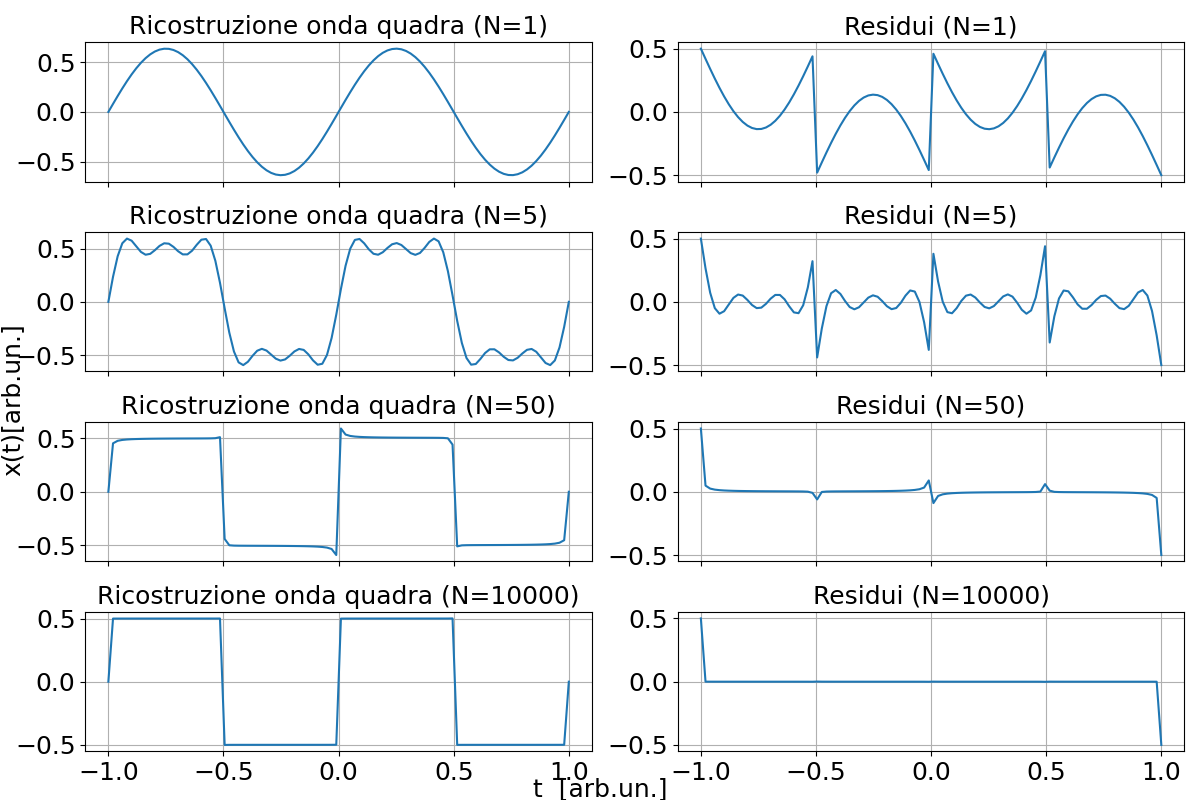
\includegraphics[width=1.2\textwidth]{fousquarewave1e2.png} % Replace with your image name
            \caption{A sinistra ricostruzione numerica dell'onda quadra Eq.($\ref{eq:quadra}$) su
                    due periodi con cento punti.
                    A destra residui tra onda analitica e la ricostruzione.
                    N è il numero a cui è stata troncata la serie.}
            \label{fig:quadra1e2}
        \end{figure}

        \begin{equation}
            x(t) = \sum_{k=1,3,5...}^{\infty} \frac{2}{k\pi}\sin\left(k\omega t\right)
            \label{eq:quadra}
        \end{equation}

        In Fig($\ref{fig:quadra1e2}$) e Fig($\ref{fig:quadra1e5}$) sono mostrate due ricostruzioni
        numeriche dell'onda quadra.
        All'aumentare dei termini $N$ della serie diminuisce la distranza tra onda analitica e serie 
        di seni.

        Si osserva che nel caso di Fig($\ref{fig:quadra1e2}$), la quale ha una risoluzione 
        peggiore, la deformazione dell'onda quadra assomiglia a quanto visto nelle esperienze 
        pratiche di laboratorio con l'oscilloscopio quando si usa il generatore di funzioni a
        frequenze sufficientemente alte: forse questo rivela qualcosa sul funzionamento del generatore
        di funzioni.\\

        \begin{figure}[H]
            \centering
            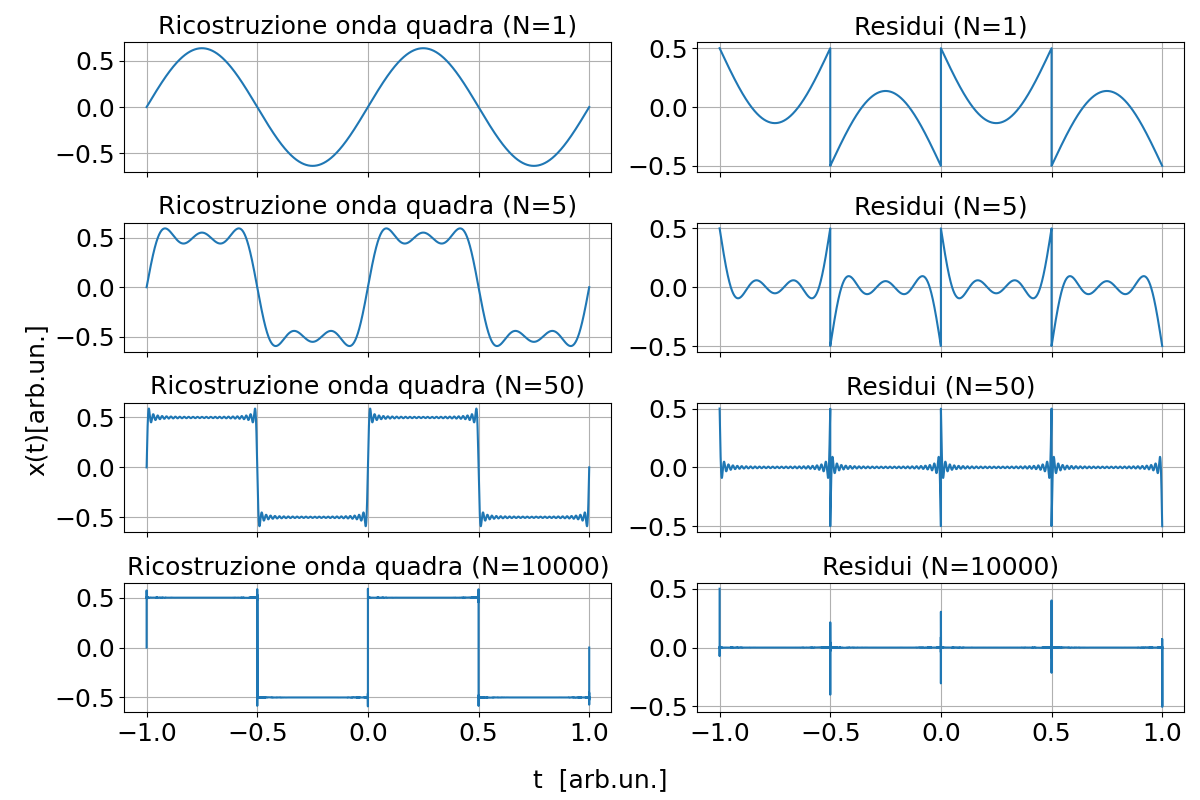
\includegraphics[width=1.2\textwidth]{fousquarewave1e5.png} % Replace with your image name
            \caption{A sinistra ricostruzione numerica dell'onda quadra Eq.($\ref{eq:quadra}$) su
                    due periodi con centomila punti.
                    A destra residui tra onda analitica e la ricostruzione.
                    N è il numero a cui è stata troncata la serie.}            \label{fig:quadra1e5}
        \end{figure}  
        
        
        Si osserva che la presenza di lati obliqui nei transienti è conseguenza di un sottocampionamento
        della mia ricostruzione, questo comporta che non c'è miglioramento all'aumentare dei termini 
        della serie.

        I residui nei punti iniziali e i transienti non si annullano mai: in corrispondenza di ognuno di
        questi punti si trovano dei picchi.




    \subsection{Forme d'onda triangolari}
        Un'onda triangolare alternata pari con ampiezza picco-picco unitaria e fase nulla è descitta dalla
        dall' Eq.($\ref{eq:triangolare}$).
        \begin{equation}
            x(t) = \sum_{k=1,3,5...}^{\infty} \left(\frac{2}{k\pi}\right)^{2}\cos\left(k\omega t\right)
            \label{eq:triangolare}
        \end{equation}


        \begin{figure}[H]
            \centering
            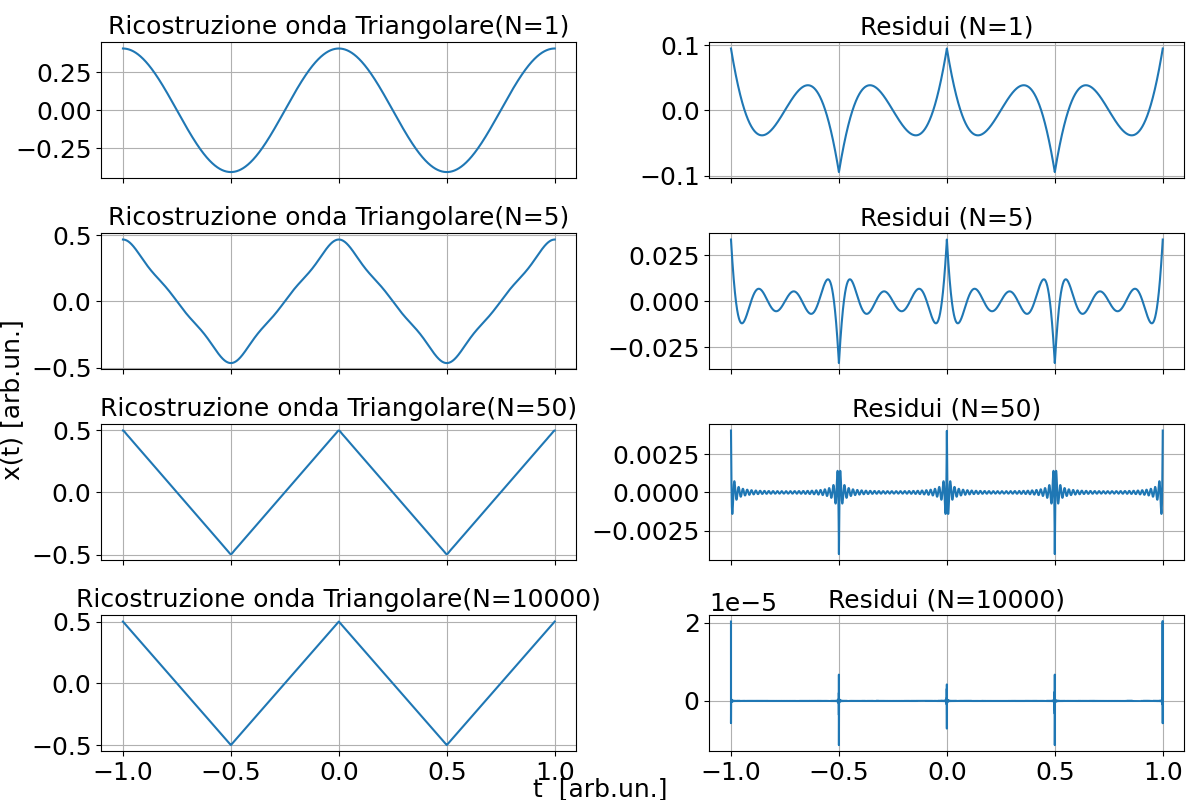
\includegraphics[width=1.2\textwidth]{foutriawave1e5.png} % Replace with your image name
            \caption{A sinistra ricostruzione numerica dell'onda triangolare
             Eq.($\ref{eq:triangolare}$)su due periodi con centomila punti.
            A destra residui tra onda analitica e la ricostruzione.
            N è il numero a cui è stata troncata la serie. }
            \label{fig:trian1e5}
        \end{figure}
        Similmente a quanto accade per l'onda quadra, anche in questo caso, nei punti 
        in cui la derivata è discontinua e nei punti al bordo non c'è convergenza come si 
        può vedere dai grafici dei residui in Fig.($\ref{fig:trian1e5}$) e Fig.($\ref{fig:trian1e2}$).
        Anche solo qualitativamente si osserva a entrambe le risolizioni che la convergenza all'onda
        analitica è più rapida dell'onda quadra, una migliore discussione di ciò avverrà in
        Sez.($\ref{sez:residui}$).
        \begin{figure}[H]
            \centering
            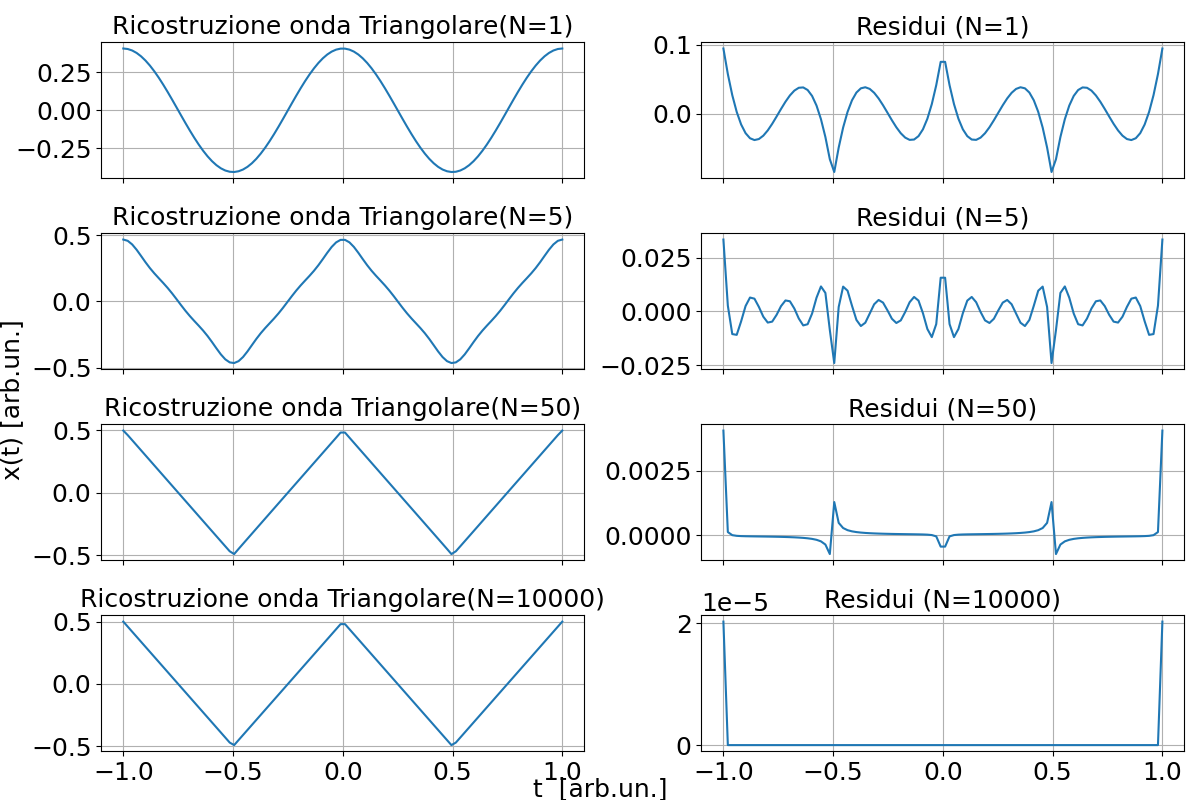
\includegraphics[width=1.2\textwidth]{foutriawave1e2.png} % Replace with your image name
            \caption{A sinistra ricostruzione numerica dell'onda triangolare
            Eq.($\ref{eq:triangolare}$)su due periodi con cento punti.
           A destra residui tra onda analitica e la ricostruzione.
           N è il numero a cui è stata troncata la serie. }
            \label{fig:trian1e2}
        \end{figure}        
        
        Per quanto riguarda l'utilizzo di diverse risoluzioni nei grafici, l'impiego di una risoluzione 
        minore comporta problemi nella convergenza solo nei punti iniziali e non nei punti di transiente,
        l'impiego di una risoluzione maggiore fa osservare dei picchi nei residui in prossimità dei transienti.
        Chiaramente non mettere i punti di picco tra i punti che vengono campionati 
        comporta una deformazione della forma d'onda graficata che non viene osservata 
        nei residui.
        \textbf{Considerazione azzardata}: questo accade perché "moralmente" se prima la mancata convergenza in certi 
        punti era un problema "puntuale", in quanto nel caso dell'onda quadra la funzione è discontinua, 
        ora la causa del problema è "locale", in quanto la discontinuità della forma d'onda analitica 
        si ha nella derivata prima.




    \subsection{Verifica di convergenza della serie}
    \label{sez:residui}
       
        La serie di Fourier delle rispettive onde dovrebbe convergere integralmente alle funzioni analitiche.
        La velocità di convergenza rispetto al numero di iterazioni
        è diversa per le forme d'onda come si può vedere in Fig.($\ref{fig:res1}$).\\ 
        Tuttavia nel caso dell'onda quadra si osserva un comportamento inaspettato:
        quando il campionamento avviene su numero sufficientemente
        piccolo di periodi,  non c'è più convergenza integrale tra la funzione semplice definita sugli 
        intervalli dalla serie di Fourier:con ogni probabilità questo è dovuto al transiente che non è 
        adeguatamente approssimato.
        Inoltre,per entrambe le onde compiono delle oscillazioni dei residui che si
        smorzano nella coda all'aumentare delle iterazioni come 
        si può vedere in Fig.($\ref{fig:res2}$).
        

        \begin{figure}[H]
            \centering
            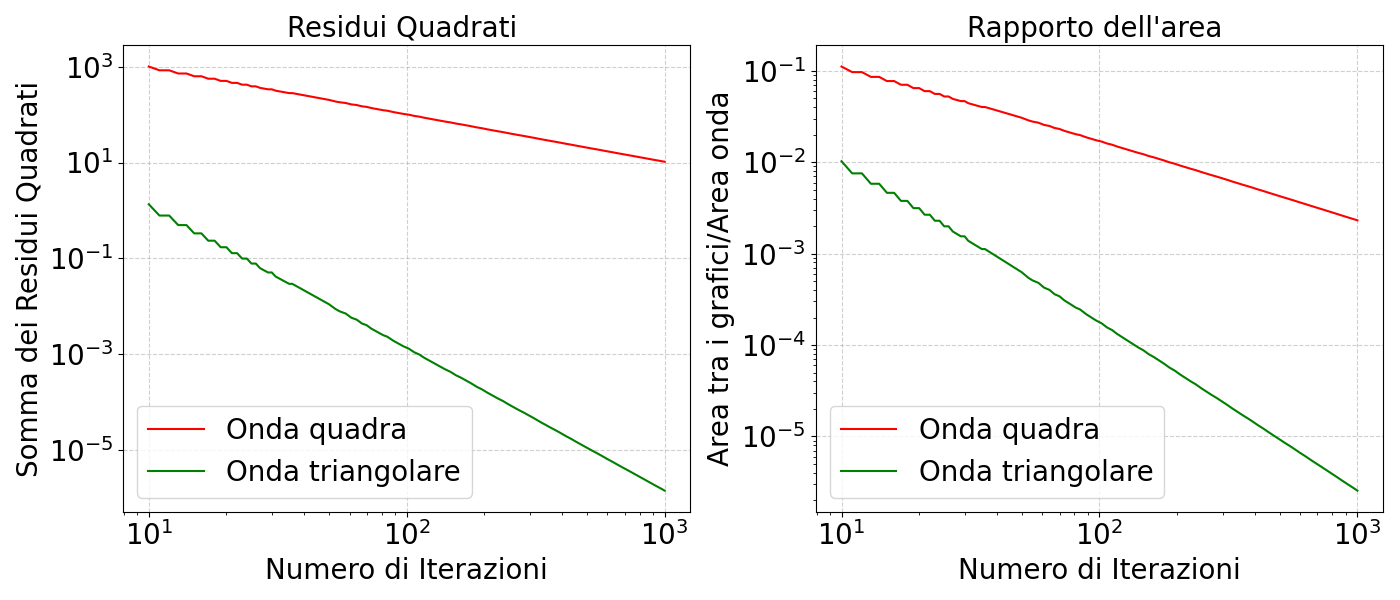
\includegraphics[width=1.2\textwidth]{residuals1.png} % Replace with your image name
            \caption{Nella figura simulazione numerica sono stati usati cento milioni di campionamenti presi tra due periodi.}
            \label{fig:res1}
        \end{figure}

      

        \begin{figure}[H]
            \centering
            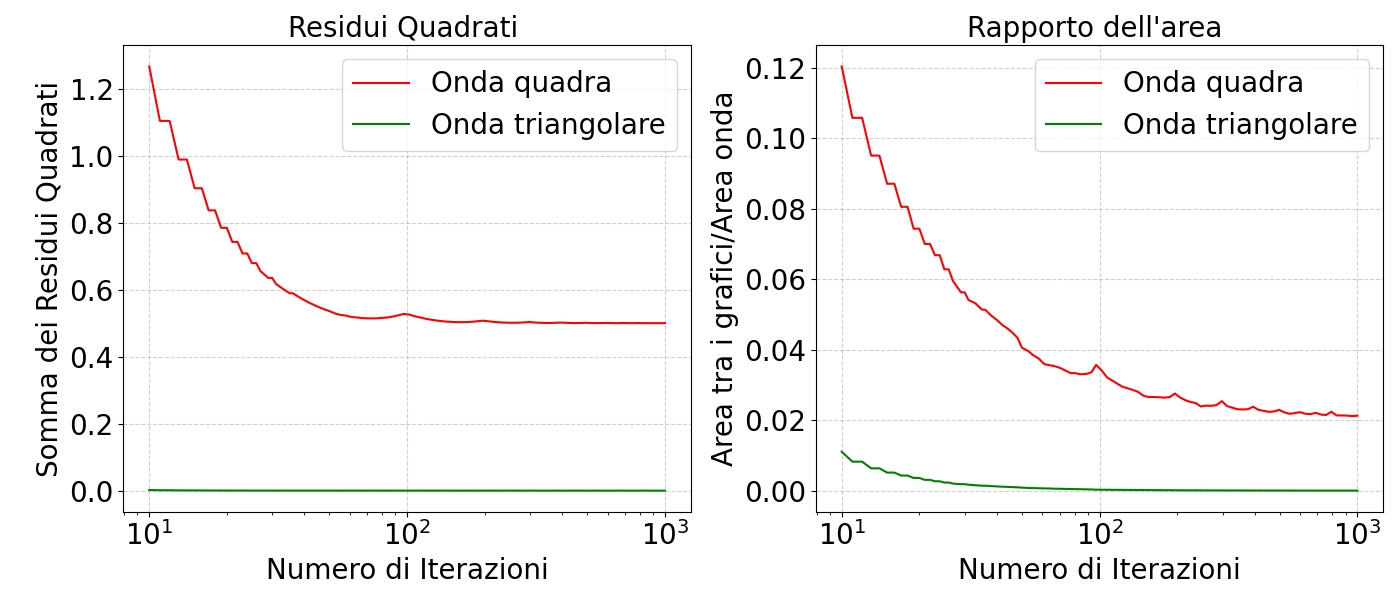
\includegraphics[width=1.2\textwidth]{residuals2.png} % Replace with your image name
            \caption{Nella figura simulazione numerica sono stati usati 100 campionamenti presi tra due periodi.}
            \label{fig:res2}
        \end{figure}

    \subsection{Treni di impulsi}
    Un treno di impulsi pari con ampiezza picco-picco unitaria e fase nulla è descitta dalla
    dall' Eq.($\ref{eq:ciufciuf}$).

    \begin{equation}
        x(t) = \sum_{k=1,3,5...}^{\infty} \left(\frac{2}{k\pi}\right)\sin\left(k\pi\delta\right)\sin\left(k\omega t\right)
        \label{eq:ciufciuf}
    \end{equation}
    Come si può vedere in Fig.($\ref{fig:ciufciuf1} $) e in Fig.($\ref{fig:ciufciuf2} $)
    si possono fare le stesse identiche osservazioni fatte in Sez(\ref{sez:quadra}).
    \begin{figure}[H]
        \centering
        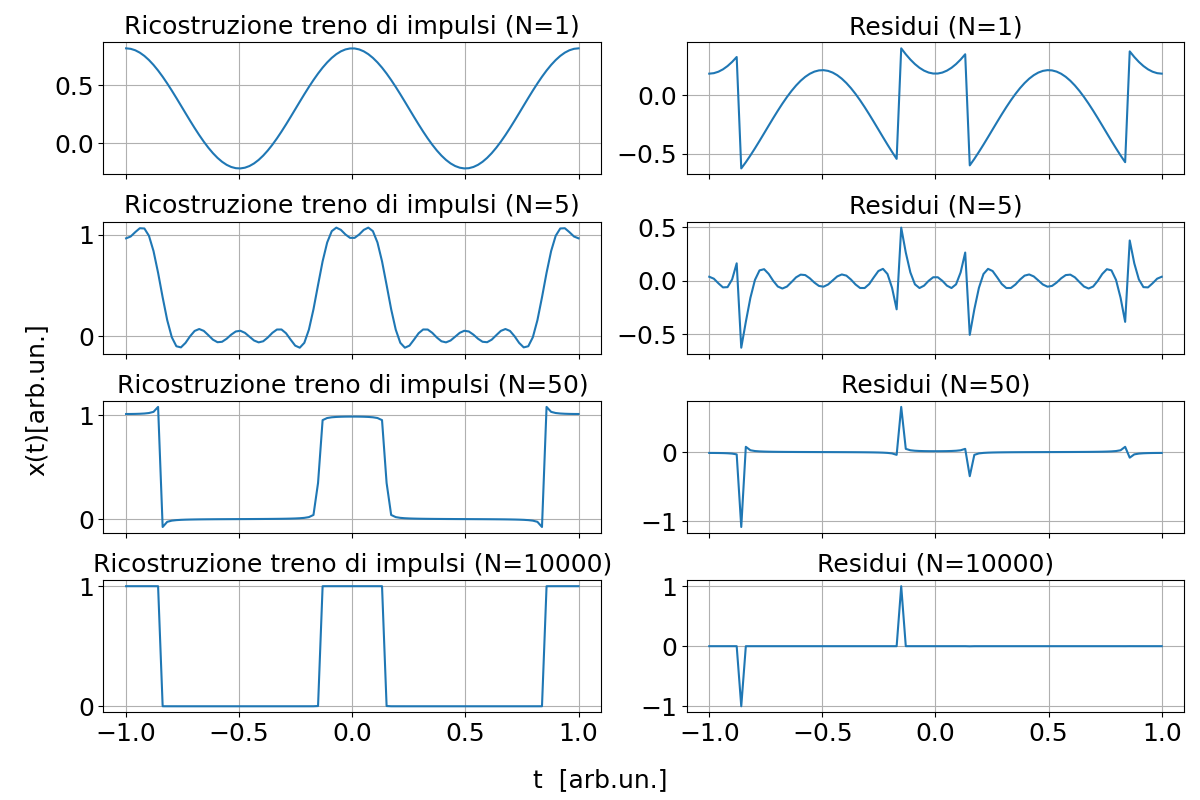
\includegraphics[width=1.2\textwidth]{foupulsetrainwave1e2.png} % Replace with your image name
        \caption{A sinistra ricostruzione numerica dell'onda triangolare
        Eq.($\ref{eq:ciufciuf}$)su due periodi con cento punti.
        A destra residui tra onda analitica e la ricostruzione.
        N è il numero a cui è stata troncata la serie. }
        \label{fig:ciufciuf1}
    \end{figure}

    \begin{figure}[H]
        \centering
        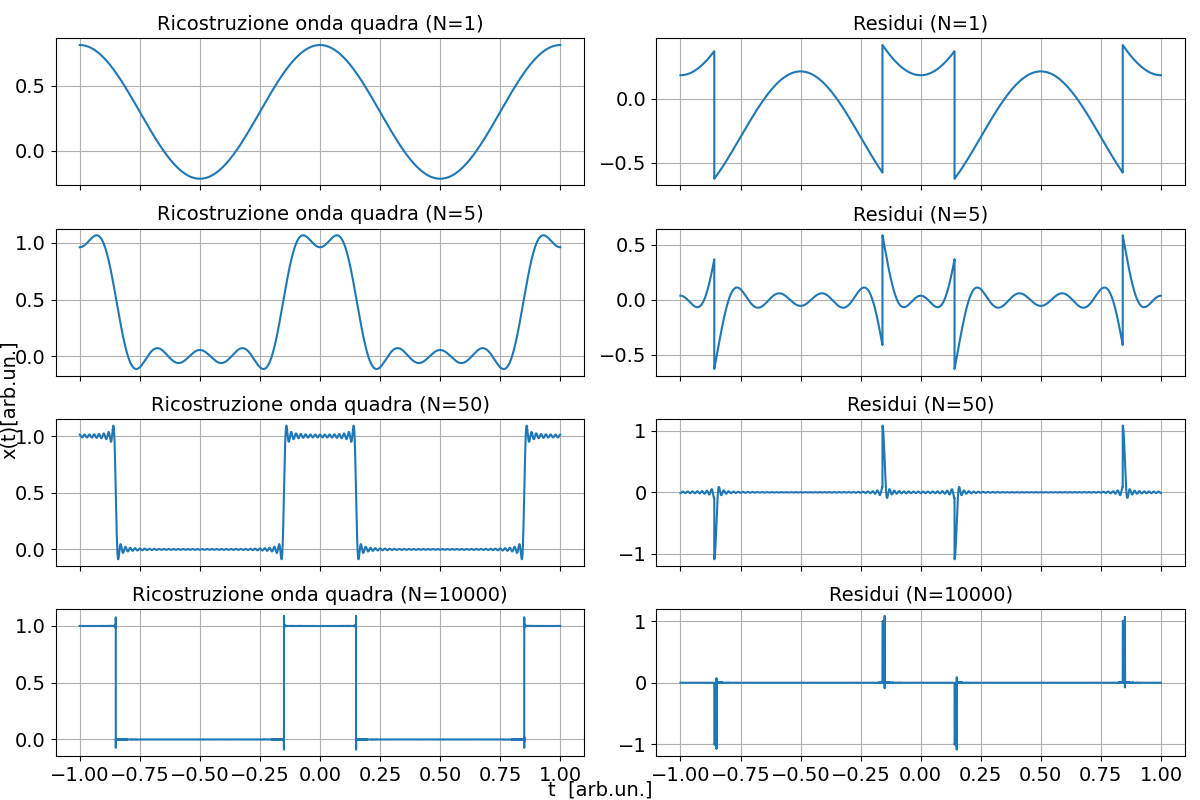
\includegraphics[width=1.2\textwidth]{foupulsetrainwave1e5.png} % Replace with your image name
        \caption{A sinistra ricostruzione numerica dell'onda triangolare
        Eq.($\ref{eq:ciufciuf}$)su due periodi con centomila punti.
        A destra residui tra onda analitica e la ricostruzione.
        N è il numero a cui è stata troncata la serie. }
        \label{fig:ciufciuf2}
    \end{figure}


        
        
    
%%%%%%%%%%%%%%%%
%
%Effetto della frequenza della forma d'onda in ingresso
%Influenza della frequenza di taglio dell'integratore
%%%%%%%%%%%%%%%%%%%%%%%%%%%%%%%%%%
\section{Filtro passa basso e filtro passa alto}
Un filtro passa basso di frequenza di taglio $f_T$, che riceve un segnale di 
frequenza angolare $\omega$,lo riscala di un fattore $G$ e lo sfasa di un 
angolo $\phi$ come dato da Eq.($\ref{eq:lpf}$).
    \begin{equation}
        f = \frac{\omega}{2\pi}, \quad 
        G(f) = \frac{1}{\sqrt{1 + \left(\frac{f}{f_T}\right)^2}}, \quad 
        \phi = \arctan\left(\frac{-f}{f_T}\right)
        \label{eq:lpf}
    \end{equation}
Un filtro passa alto di frequenza di taglio $f_T$, che riceve un segnale di 
frequenza angolare $\omega$,lo riscala di un fattore $G$ e lo sfasa di un 
angolo $\phi$ come dato da Eq.($\ref{eq:hpf}$).
    \begin{equation}
        f = \frac{\omega}{2\pi}, \quad 
        G(f) = \frac{1}{\sqrt{1 + \left(\frac{f_T}{f}\right)^2}}, \quad 
        \phi = \arctan\left(\frac{f_T}{f}\right)
        \label{eq:hpf}
    \end{equation}

Dunque le equazioni per le onde passanti per ciascuno dei filtri si trovano
moltiplicando ciascun termine della sommatoria per il rispettivo 
$G \left( k\omega,f_T\right)$ e sommando il termine $\phi \left( k\omega,f_T\right)$ 
all'interno della sinusoide o cosinusoide.
      

    
    \subsection{Onda quadra}
        Riporto la forma d'onda della cosinusoide integrata in . 
            \begin{figure}[H]
                \centering
                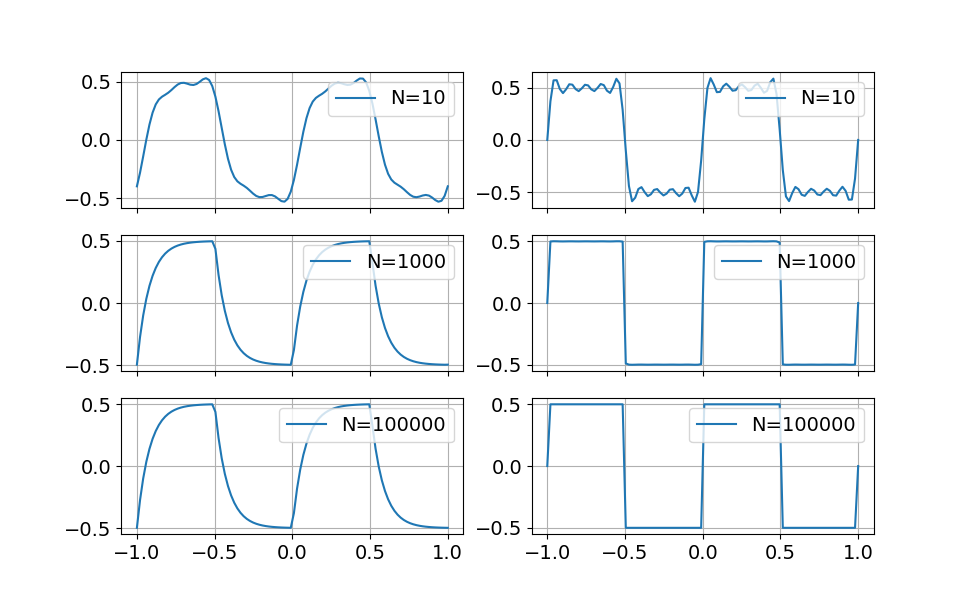
\includegraphics[width=1.2\textwidth]{fousharkfins.png} % Replace with your image name
                \caption{}
                \label{fig:shark1}
            \end{figure}

    \subsection{Onda triangolare}
    \subsection{Treno di impulsi}




\section{Filtro passa banda}


\section{Best fit dei dati acquisiti con Arduino}
    \subsection{Onda quadra}
    \subsection{Onda a pinna di squalo}
    \subsection{Onda sinusoidale}
    \subsection{Onda triangolare}



\section{Simulazione numerica dei grafici guadagno vs frequenza}
    \subsection{Integratore con forma d'onda quadra in ingresso}
        \subsubsection{Contestualizzazione dei risultati sperimentali}
    \subsection{Integratore con forma d'onda triangolare in ingresso}
        \subsubsection{Contestualizzazione dei risultati sperimentali}



\section{Simulazioni facoltative}
    \subsection{Derivatore con forma d'onda a scelta in ingresso}
    \subsection{Distorsione di una forma d'onda quadra osservata con accoppiamento AC}
    \subsection{Forma d'onda quadra con duty cycle variabile e filtro passa-basso}
        \subsubsection{Effetti del filtro passa-basso su un treno di impulsi}
    \subsection{Altre simulazioni e confronti con dati sperimentali}

\end{document}